\section*{Learning Objectives}

\begin{itemize}
\item Understand basis vectors and why they are so useful.
\item Coming to grips with eigenvalues and eigenvectors. 
\end{itemize}

\section*{Outcomes} 
\begin{itemize}
\item Basis vectors provide a compact means of defining a subspace
\item Every vector in a subspace can be written as a linear combination of a set of basis vectors
\item Because of the Gram-Schmidt Algorithm, once we find any basis for a subspace, we know how to generate one where the vectors are orthonormal
\item The dimension of a subspace is the number of vectors in any basis. 
\item Even though basis vectors for a subspace are not unique, the number of vectors in a basis is unique
\item Learn the \texttt{$\backslash$} command in Julia for solving linear systems of equations. It will automatically use the best method available when solving the equation, such as LU or QR, without you having to think about it.

\item A non-zero vector $v$ is an eigenvector of a square matrix $A$ if there exists a number $\lambda$ such that $Av = \lambda v$. The number $\lambda$ is called an eigenvalue. We will sometimes use e-value and e-vector for short.
\item An $n \times n$ matrix has $n^2$ entries. It seems positively amazing that there can exist vectors such that multiplying $v$ on the left by $A$ is the same as multiplying $v$ by a scalar, $\lambda$. 
\item Such an amazing property must have huge consequences for applied Linear Algebra, and it does!
\item  We'll learn the \texttt{eigen()} command/function in Julia to compute eigenvalues and eigenvectors of a matrix.
\end{itemize}

\vspace*{1cm}

\textbf{Either download Lab8 from our Canvas site or open up a Jupyter notebook so that you can enter code as we go. It is suggested that you have line numbering toggled on.}  

\newpage

This lab goes all in on basis vectors. 

\section{Basis Vectors, Linear Independence, and Span}

\begin{tcolorbox}[sharp corners, colback=green!30, colframe=green!80!blue, title=\textbf{\Large Basis Vectors and Dimension}]
Suppose that $V$ is a subspace of $\real^n$. Then $\{ v_1, v_2, \ldots, v_k\}$ is a \textbf{basis for} ${\bf V}$ if
\begin{enumerate}
    \item the set $\{ v_1, v_2, \ldots, v_k\}$ is linearly independent, and 
    \item $\spanof{v_1,  v_2,\ldots, v_k}=V$, that is, every vector in $V$ can be expressed as a linear combination of $\{ v_1, v_2, \ldots, v_k\}$.
\end{enumerate}

The \textbf{dimension of} ${\bf V}$ \textbf{is} ${\bf k}$, the number of basis vectors.\\

We note that the above definition applies to $\real^n$ \textbf{because} $\real^n$ is a subset of itself and it is closed under linear combinations. In particular, $\real^n$ has dimension $n$, or we say that $\real^n$ is an $n$-dimensional vector space.
\end{tcolorbox}

\begin{rem} We can check \textbf{linear independence} in two ways: define $A:=\begin{bmatrix} v_1 & v_2 & \cdots & v_k\end{bmatrix}$ and 
\begin{itemize}
    \item check $\det(A^\top \cdot A)$ is not equal to zero, or even better, \item do the LU factorization of $A^\top \cdot A$ and check that there are no zeros on the diagonal of $U$. 
\end{itemize}

 For the \textbf{span condition}, we want to check if a vector $v$ can be written as a \textbf{linear combination} of  $\{v_1, v_2, ..., v_k\}$ or not. This is really asking if the equation
$$c_1 v_1 + c_2 v_2 + \cdots + c_k v_k = \underbrace{\begin{bmatrix} v_1 & v_2 & \cdots & v_k\end{bmatrix}}_{A} \underbrace{\begin{bmatrix} c_1\\ c_2 \\ \vdots \\c_k\end{bmatrix}}_{c} = v  $$
has a solution or not. In Chapter 8.2 of our textbook, we showed a cool way for checking this condition and for finding a solution, if it exists. We'll review that shortly. 
\end{rem}

\begin{lstlisting}[language=Julia,style=mystyle]
using LinearAlgebra

# Determine linear independence 
function is_independent(A, aTol=1e-10)
    if false # change to true to use this version of the test
        test = det(A'*A) # non-zero means columns of A are independent
    else 
        F = lu(A'*A, check=false)
        test = minimum(abs.(diag(F.U))) # non-zero means columns of A are independent
    end
    return !isapprox(test, 0.0, atol=aTol) # return true when test
                                # is large enough in magnitude
end
\end{lstlisting}
\textbf{Output} 
\begin{verbatim}
is_independent (generic function with 2 methods)
\end{verbatim}

\begin{lstlisting}[language=Julia,style=mystyle]
# Check e1 and e2 are linearly independent, where
e1 = [0; 1]
e2 = [1; 0]
A = [e1 e2]
@show is_independent(A), size(A)
#
using Random
Random.seed!(2000)
A = randn(12, 12) # random square matrix
@show is_independent(A), size(A)
#
A = randn(12, 15) # random wide matrix (more columns than rows)
@show is_independent(A), size(A)
#
#
A = randn(12, 8) # random tall matrix (more rows than columns)
@show is_independent(A), size(A); # semicolon suppresses repeated output
\end{lstlisting}
\textbf{Output} 
\begin{verbatim}
(is_independent(A), size(A)) = (true, (2, 2))
(is_independent(A), size(A)) = (true, (12, 12))
(is_independent(A), size(A)) = (false, (12, 15))
(is_independent(A), size(A)) = (true, (12, 8))
\end{verbatim}

\begin{tcolorbox}[sharp corners, colback=green!30, colframe=green!80!blue, title=\textbf{\large Least Squares Solutions to Linear Equations}]
Here are the main results on solutions to $Ax=b$ that minimize the squared error $||Ax-b||^2$.
\begin{enumerate}
\renewcommand{\labelenumi}{(\alph{enumi})}
\setlength{\itemsep}{.2cm}

\item $A^\top A$ is invertible if, and only if, the columns of $A$ are linearly independent.

\item If $A^\top A$ is invertible, then there is a unique vector $x^\ast \in \real^m$ achieving $\min_{x \in \real^m } ||Ax-b ||^2$ and it satisfies the equation
\begin{equation}
    \label{eq:LeastSquaresSolution}
    \left(A^\top A \right) x^\ast = A^\top b.
\end{equation}
\item Therefore, if $A^\top A$ is invertible, 
\begin{equation}
    \label{eq:ThmLeastSqaredErrorSolution}
  x^\ast = (A^\top A)^{-1} A^\top b  \iff  x^\ast = \argmin_{x \in \real^m} ||Ax-b ||^2 \iff \left(A^\top A \right) x^\ast = A^\top b.
\end{equation}
\end{enumerate}
As you might guess by now, your instructors prefer that for large systems of equations, you solve \eqref{eq:LeastSquaresSolution} to obtain the least squares solution and avoid doing the inverse. For small systems, we'll cut you some slack.
\end{tcolorbox}

\vspace*{.2cm}

\begin{tcolorbox}[title=\textbf{\large Useful Remark for Solving Tall Linear Equations}] Suppose that $A$ is a ``tall matrix'' (more rows than columns) and suppose that $Ax=b$ has a solution (hence, $b$ is a linear combination of the columns of $A$). Then, if the columns of $A$ are linearly independent, you can compute the solution using \eqref{eq:LeastSquaresSolution} and the squared error will be zero, meaning $x^\ast$ really is a solution to the equation because $$\text{the squared error is zero} \iff ||A x^\ast - b||^2 = 0 \iff ||A x^\ast - b|| = 0 \iff A x^\ast - b=0 \iff A x^\ast = b.$$ 
\end{tcolorbox}


\vspace*{.2cm}



\begin{rem}
The matrix $(A^\top \cdot A)$ is square and invertible when $\{v_1, v_2, ..., v_k\}$ is linearly independent. Hence we can solve for $c$ by $(A^\top \cdot A) c = A^\top w$. This equation can be solved in many ways: 
\begin{itemize}
    \item using the inverse command, which we dislike; 
    \item using LU or QR Factorization, which we love a lot; or 
    \item \textbf{using a new Julia trick involving the backslash command}: $c = (A'*A)\backslash (A'*w)$ where here, the backslash command solves the equation $(A^\top \cdot A) c = A^\top w$ using what Julia finds to be the most efficient means at its disposal, typically one of LU or QR, but not always.
\end{itemize}
\end{rem}

\vspace*{.2cm}

\begin{exercise} Write a function to express a given vector $w$ as a linear combination of basis vectors $\{v_1, v_2, ..., v_k\}$, that is,
$$w = c_1 v_1 + c_2 v_2 + \cdots + c_k v_k \iff A c = w $$
where $A:=\begin{bmatrix} v_1 & v_2 & \cdots & v_k\end{bmatrix}$ and $c = \begin{bmatrix} c_1\\ c_2 \\ \vdots \\c_k\end{bmatrix}$.
\end{exercise}

\textbf{Solution:}

\begin{lstlisting}[language=Julia,style=mystyle]
function expressLinearCombination(A, w, aTol=1e-4)
    # Assume columns of V are linearly independent
    c = (A'*A)\(A'*w) #  (A'*A) c = A'*w
    # You end here
    if norm(A*c-w) > aTol
        c = NaN # c = NaN will indicate that no solution exists
    end
    return c
end
\end{lstlisting}
\textbf{Output} 
\begin{verbatim}
expressLinearCombination (generic function with 2 methods)
\end{verbatim}

\begin{lstlisting}[language=Julia,style=mystyle]
# A is a tall matrix, meaning more rows than columns.
A = [ -0.432768    0.038062   -0.187462
 -0.0418031  -0.787585    0.0321116
  0.640989   -0.036278    0.306395
  0.601849    0.11336    -0.19077
 -0.0801513   0.598622   -0.00674714
 -0.177342    0.0758032   0.912968]
w = [-0.91903  -1.52064  1.48762  0.256259  1.09685  2.71317]'
w2 = [2.24379  1.67673  0.56574  0.67676  1.74866  -22.167922]'
#
c=expressLinearCombination(A, w)
if isnan(c[1])
    println("There is no solution, and hence w is not a linear combo of columns of A")
end
@show c # should be a column vector with three components
@show  norm(A*c-w)
#
c2=expressLinearCombination(A, w2)
@show c2
if isnan(c2[1])
    println("There is no solution, and hence w2 is not a linear combo of columns of A")
end
\end{lstlisting}
\textbf{Output} 
\begin{verbatim}
c = [1.0000011718917985; 2.0000006213876516; 3.0000020275852974]
norm(A * c - w) = 2.28426074545448e-6
c2 = NaN
There is no solution, and hence w2 is not a linear combo of columns of A
\end{verbatim}

\begin{lstlisting}[language=Julia,style=mystyle]
# Run me and note that our function works to find more than 
# one linear combination at a time
c=expressLinearCombination(A, [w 2*w])
@show norm(A*c[:,1] - w), norm(A*c[:,2] - 2*w), norm(A*c-[w 2*w])
c
\end{lstlisting}
\textbf{Output} 
\begin{verbatim}
(norm(A * c[:, 1] - w), norm(A * c[:, 2] - 2w), norm(A * c - [w 2w])) =
(2.28426074540208e-6, 4.56852149080416e-6, 5.107762304797088e-6)

3×2 Matrix{Float64}:
 1.0  2.0
 2.0  4.0
 3.0  6.0
\end{verbatim}
\Qed

\section{Vector Space Coordinates and Vector Representations}

\begin{tcolorbox}[title=\textbf{\large A Basis Defines Coordinates}] Suppose that $V$ is a $k$-dimensional subspace of $\mathbb{R}^n$ with basis $\{v_1, v_2, ..., v_k\}$. We note that if $k=n$, then $V$ is all of $\mathbb{R}^n$. \\

Due to the linear independence property of a basis, each $x \in V$ can be expressed (uniquely) as a linear combination of basis vectors
$$x = c_1 v_1 + c_2 v_2 + ... + c_k v_k.$$

Stacking the coefficient $c_1, c_2, ..., c_k$ into a column vector yields
$$[x]_{\{v_1, ..., v_k\}} := \begin{bmatrix}
c_1 \\ c_2 \\ \vdots \\ c_k
\end{bmatrix},$$
which forms the \textbf{coordinates} of $x \in V$ associated to the basis $\{v_1, v_2, ..., v_k\}$.
\end{tcolorbox}

\begin{rem}  Let's consider $\mathbb{R}^2$, $\{v1=e_1, v2=e_2\}$, the so-called natural basis vectors. The span property of the vectors $\{e_1, e_2\} \subset \mathbb{R}^2$ is easy to check because, for any vector $x \in \mathbb{R}^2$, it can be written as a \textbf{linear combination} of $\{e_1, e_2\}$ per
$$
x := \begin{bmatrix} x_1 \\ x_2 \end{bmatrix}
= x_1 \begin{bmatrix} 1 \\ 0 \end{bmatrix}
+ x_2 \begin{bmatrix} 0 \\ 1 \end{bmatrix}
= x_1 e_1 + x_2 e_2.
$$

\textbf{Therefore the coordinates of $x$ associated to the basis $\{e_1, e_2\}$ are simply $(x_1, x_2)$.} With other bases, the concept of representing vectors can be more interesting. We will limit ourselves to cases that we can visualize.
\end{rem}

The following function will plot the coordinates associated with a given pair of basis vectors in $\real^2$ and plot a point that has been expressed in the given basis vectors.\\

\begin{lstlisting}[language=Julia,style=mystyle]
using Plots

# Function of ploting a 2-d vector v using basis vectors {v1, v2} in R^2
function plot_with_basis(v1, v2, v)
    t = LinRange(-4, 4, 10)
    t = collect(t)
    titre = "Basis Vectors"
    p1 = plot(t, 0.0.*t, framestyle=:origin, aspect_ratio=1, 
        title=titre, legend=false, color=:black, lw=3)
    p1 = plot!(0.0.*t, t, color=:black, lw=3)
    for k = -4:4
        X = k*v1[1] .+ t.*v2[1]
        Y = k*v1[2] .+ t.*v2[2]
        p1 = plot!(X, Y, color=:gray)
    end
    for k = -4:4
        X = k*v2[1] .+ t.*v1[1]
        Y = k*v2[2] .+ t.*v1[2]
        p1 = plot!(X, Y, color=:gray)
    end
    p1 = plot!([0,v1[1]], [0,v1[2]], arrow=true, color=:blue, lw=4)
    p1 = plot!([0,v2[1]], [0,v2[2]], arrow=true, color=:green, lw=4)
    #
    # Plot the vector v
     titre = "Vector $v"
    p2 = plot(t, 0.0.*t, framestyle=:origin, aspect_ratio=1, 
        title=titre, legend=false, color=:black, lw=3)
    p2 = plot!(0.0.*t, t, color=:black, lw=3)
    for k = -4:4
        X = k*v1[1] .+ t.*v2[1]
        Y = k*v1[2] .+ t.*v2[2]
        p2 = plot!(X, Y, color=:gray)
    end
    for k = -4:4
        X = k*v2[1] .+ t.*v1[1]
        Y = k*v2[2] .+ t.*v1[2]
        p2 = plot!(X, Y, color=:gray)
    end
    pt = v[1]*v1 + v[2]*v2
    p2 = plot!([0, v[1]*v1[1]], [0, v[1]*v1[2]], color=:blue, lw=4)
    p2 = plot!([v[1]*v1[1], v[1]*v1[1]+v[2]*v2[1]], [v[1]*v1[2], v[1]*v1[2]+v[2]*v2[2]], color=:green, lw=4)
    p2 = scatter!([pt[1]], [pt[2]], color=:red)
    plot(p1, p2, layout=(1, 2))
end
\end{lstlisting}
\textbf{Output} 
\begin{verbatim}
plot_with_basis (generic function with 1 method)
\end{verbatim}

\begin{lstlisting}[language=Julia,style=mystyle]
# We can plot a vector using the natural basis vectors
e1 = [1; 0]
e2 = [0; 1]
x = [3; 2] # means x = 3 e1 + 2 e2
plot_with_basis(e1, e2, x)
\end{lstlisting}
\textbf{Output} 
\begin{center}
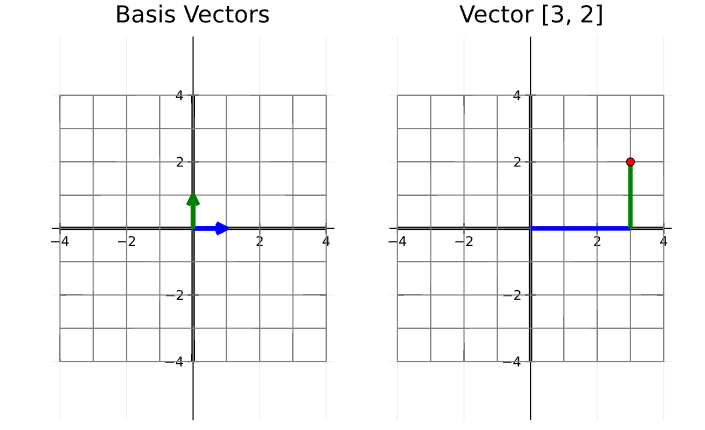
\includegraphics[width=0.6\columnwidth]{graphics/Chap08/BasisVectors_e1e2.png}
\end{center}
\begin{lstlisting}[language=Julia,style=mystyle]
# We can plot a vector x with respect to a different set of basis vectors in R^2
v1 = [1.5; -0.2]
v2 = [0.2; 1.5]
x = [3; 2] # means x = 3 v1 + 2 v2
plot_with_basis(v1, v2, x)
\end{lstlisting}
\textbf{Output} 
\begin{center}
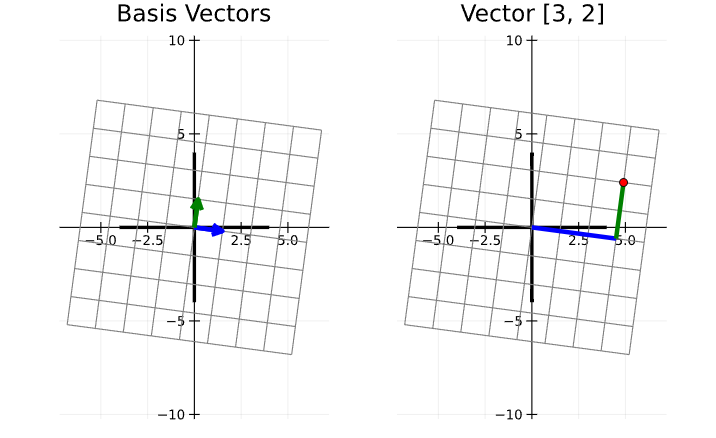
\includegraphics[width=0.6\columnwidth]{graphics/Chap08/BasisVectors_v1v2.png}
\end{center}
Next, we show an example in $\real^3$
\begin{lstlisting}[language=Julia,style=mystyle]
z(x, y) = 2x+y
x = -1:1
y = -1:1
p1=plot(x, y, z, st=:surface, legend = false)
titre = "A 2D subspace in R3. All points satisfy 0 = 2x + y - z"
pl = plot!(title = titre, xlabel="X", ylabel = "Y", zlabel="Z")
display(p1)
#
# Next, add basis vectors to the plot
A = [2 1 -1]
V = nullspace(A) # columns will be orthonormal vectors
#
v1=-V[:,1]; v2=V[:,2];
p2 = plot!([0,v1[1]], [0,v1[2]], [0,v1[3]], arrow=true, color=:blue, lw=4)
p2 = plot!([0,v2[1]], [0,v2[2]], [0,v2[3]], arrow=true, color=:green, lw=4)
titre = "Orthonormal basis vectors on our subspace"
p2 = plot!(title = titre)
display(p2)
#
# Finally, show grid lines on the plot
# In other words, show coordinate lines on the plot
t = LinRange(-1, 1, 10)
t = collect(t)
    for k = -3:3
        X = .33*k*v1[1] .+ t.*v2[1]
        Y = .33*k*v1[2] .+ t.*v2[2]
        Z = .33*k*v1[3] .+ t.*v2[3]
        p3 = plot!(X, Y, Z, color=:gray)
    end
    for k = -3:3
        X = .33*k*v2[1] .+ t.*v1[1]
        Y = .33*k*v2[2] .+ t.*v1[2]
        Z = .33*k*v2[3] .+ t.*v1[3]
        p3 = plot!(X, Y, Z, color=:gray)
    end
titre = "Basis vectors define coordinate lines on subspace"
p3 = plot!(title = titre)
display(p3)
\end{lstlisting}
\textbf{Output} 

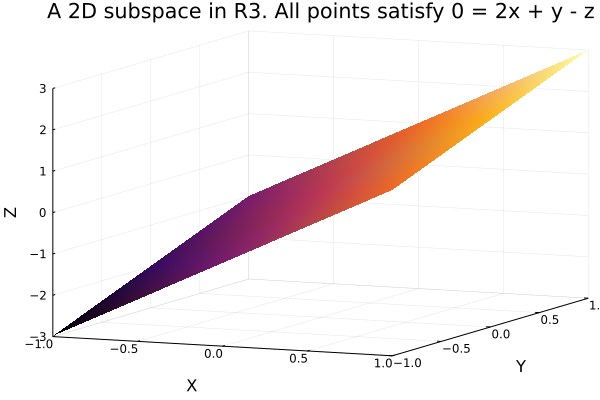
\includegraphics[width=0.45\columnwidth]{graphics/Chap08/2DPlane.png} \hspace*{.2cm}
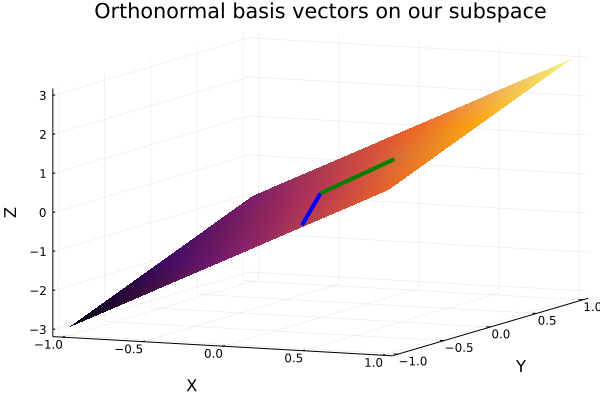
\includegraphics[width=0.45\columnwidth]{graphics/Chap08/2DPlaneWithBasisVectors.png}
\begin{center}
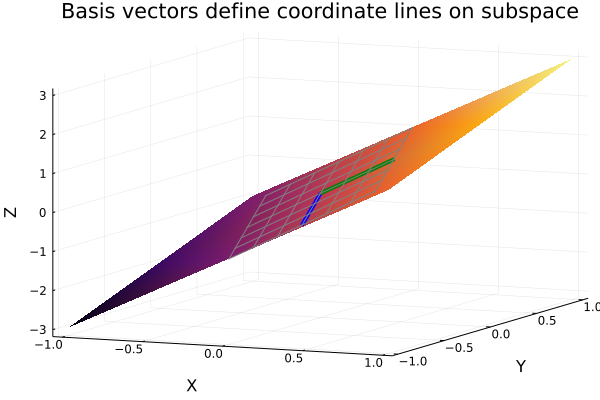
\includegraphics[width=0.45\columnwidth]{graphics/Chap08/2DPlaneWithCoordinateLines.png}
\end{center}

\begin{exercise} Find a basis for the subspace of $\mathbb{R}^3$ defined by
$$V:= \{ (x, y, z) | z = 3x + 2y\}.$$
\end{exercise}

\textbf{Solution:}

\begin{lstlisting}[language=Julia,style=mystyle]
## BEGIN YOUR SOLUTION HERE
A = [3 2 -1]
Vbasis = nullspace(A)
### END YOUR SOLUTION HERE
\end{lstlisting}
\textbf{Output} 
\begin{verbatim}
3×2 Matrix{Float64}:
 -0.534522   0.267261
  0.841427   0.0792865
  0.0792865  0.960357
\end{verbatim}

\begin{lstlisting}[language=Julia,style=mystyle]
# Friendly self test
T1 = @assert isapprox(A*Vbasis, [0 0], atol=1e-6)
println("all nothings means likely correct")
[T1]
\end{lstlisting}
\textbf{Output} 
\begin{verbatim}
all nothings means likely correct

1-element Vector{Nothing}:
 nothing
\end{verbatim}

\Qed

\section{Eigenvectors and Eigenvalues}

In ROB 101, we are limiting ourselves to real eigenvalues and real eigenvectors. The Appendix of our textbook covers the case of complex eigenvalues and complex eigenvectors.

\begin{tcolorbox}[title=\textbf{\Large Eigen Stuff: Incomplete Definition but Good Enough to Get us Started}]
 Let $A$ be an $n\times n$ matrix with real coefficients. A scalar $\lambda \in \real$ is an \textbf{eigenvalue} of $A$, if there exists a non-zero vector $v \in \real^{n}$ such that $A  v=\lambda v$.  Any such vector $v$ is called an \textbf{eigenvector} associated with $\lambda$. \\
 
 We note that if $v$ is an eigenvector, then so is $\alpha v$ for any $\alpha \neq 0$, and therefore, eigenvectors are not unique. The true definition is given in the Appendix of our textbook.
\end{tcolorbox}

\begin{tcolorbox}[title=\textbf{\Large Finding Eigenvectors and Eigenvalues with Julia}]
We do not care to compute eigenvalues or eigenvectors by hand in ROB 101. We use Julia, instead!

\begin{lstlisting}[language=Julia,style=mystyle]
Random.seed!(876543212345678);
A=randn(4,4)
A=A'*A # It's a fact that symmetric matrices have real eigenvalues
E=eigen(A)
@show E.values
E.vectors
\end{lstlisting}
\textbf{Output} 
\begin{verbatim}
E.values = [0.06287200462929299, 0.6813033999332612, 2.9738855645273268, 
4.4839915456638]

4 x 4  Matrix{Float64}:
  0.339074   0.0385456  -0.71411   -0.61122
  0.551488   0.528452   -0.226828   0.604275
 -0.191731   0.824533    0.318536  -0.426521
  0.737651  -0.19849     0.58063   -0.281676
\end{verbatim}
\end{tcolorbox}

In the above, each column of \texttt{E.vectors} contains an e-vector of the matrix $A$. In fact, for $1 \le i \le \text{ number of columns of A}$, we have
$$A*E.vectors[:,i] = E.values[i] *  E.vectors[:,i]  $$

\begin{tcolorbox}[sharp corners, colback=green!30, colframe=green!80!blue, title=\textbf{\Large When the Eigenvalues are Real and Distinct, the Eigenvectors form a Basis of $\real^n$}]
Let $A$ be an $n \times n$ matrix with real coefficients. If the eigenvalues $\{ \lambda_1,\ldots, \lambda_n \}$ are real and \textbf{distinct}, that is, $\lambda_i \neq \lambda_j $ for all $1 \le i \neq j \le n$, then the eigenvectors $\{ v_1,\ldots,v_n \}$ are real and provide a basis of $\real^n.$\\

The case of complex eigenvalues and eigenvectors is covered in the Appendix of our textbook. An interesting tidbit is that symmetric matrices always have real eigenvalues. Moreover, their eigenvectors can always be selected to form an orthogonal matrix.
\end{tcolorbox}

\begin{lstlisting}[language=Julia,style=mystyle]
using Random
Random.seed!(8765432123456)

# Symmetric matrices have real eigenvalues
A = randn(4, 4)
A = A+A'

# Compute eigenvalues and eigenvectors
E = eigen(A)
@show E.values
E.vectors
\end{lstlisting}
\textbf{Output} 
\begin{verbatim}
E.values = [-3.6258168896748075, -0.5790181480494843, 0.10365049366010881,
1.4790240511628157]

4×4 Matrix{Float64}:
 0.376015   0.798978  -0.133442   0.449933
 0.53203    0.223155   0.10347   -0.81021
 0.586088  -0.478348  -0.630802   0.17255
 0.481724  -0.288131   0.757348   0.333687
\end{verbatim}

Next we show that the eigenvectors computed by Julia are orthonormal. Now, because $E.vectors'*E.vectors = I_{4 \times 4}$, we also see that the vectors are linearly independent. Why? Because $\det(I)=1 \neq 0$.\\

\begin{lstlisting}[language=Julia,style=mystyle]
cleanUp(E.vectors'*E.vectors)
\end{lstlisting}
\textbf{Output} 
\begin{verbatim}
4×4 Matrix{Float64}:
 1.0  0.0  0.0  0.0
 0.0  1.0  0.0  0.0
 0.0  0.0  1.0  0.0
 0.0  0.0  0.0  1.0
\end{verbatim}

\vspace*{.2cm}
\begin{tcolorbox}[sharp corners, colback=green!30, colframe=green!80!blue, title=\textcolor{red}{\Large \bf Eigenvalues and Eigenvectors Explain how a Square Matrix acts on a Vector}]
Let $A$ be an $n \times n$ real matrix with real eigenvalues $\{ \lambda_1,\ldots, \lambda_n \}$ that are \textbf{distinct}, that is, $\lambda_i \neq \lambda_j $ for all $1 \le i \neq j \le n$. It then follows that the eigenvectors $\{ v_1,\ldots,v_n \}$ provide a basis for $\real^n.$ Let $x\in \real^n$ be arbitrary and write it as a linear combination of the basis of eigenvectors
\begin{equation}
    \label{eq:xExpandedEigenBasis}
    x = \alpha_ 1 v_1 + \alpha_2 v_2 + \cdots + \alpha_n v_n.
\end{equation}
Then because $Av_i = \lambda_i v_i$,
\begin{equation}
    \label{eq:xExpandedEigenBasisA}
   A x = \alpha_ 1 \lambda_1 v_1 + \alpha_2 \lambda_2 v_2 + \cdots +\alpha_n  \lambda_n v_n.
\end{equation}
If we apply $A$ to both sides of \eqref{eq:xExpandedEigenBasisA}, we obtain
\begin{equation}
    \label{eq:xExpandedEigenBasisA2}
    \begin{aligned}
       A^2 x &= \alpha_ 1 \lambda_1 A v_1 + \alpha_2 \lambda_2 A v_2 + \cdots +\alpha_n  \lambda_n Av_n \\
       &= \alpha_ 1 (\lambda_1)^2 v_1 + \alpha_2 (\lambda_2)^2  v_2 + \cdots +\alpha_n  (\lambda_n)^2 v_n,
    \end{aligned}
\end{equation}
where $A^2:= A \cdot A$ and we have used again, $A v_i = \lambda_i v$. 
Moreover, using this fact iteratively yields that, for all $k \ge 2$,
\begin{equation}
    \label{eq:xExpandedEigenBasisB}
   A^k x = \alpha_ 1 (\lambda_1)^k v_1 + \alpha_2 (\lambda_2)^k v_2 + \cdots +\alpha_n  (\lambda_n)^k v_n.
\end{equation}

\end{tcolorbox}
\vspace*{.2cm}

Equation \eqref{eq:xExpandedEigenBasisB} may not seem very important at first glance, but is is really a gold mine! We next illustrate this for the special case that $x = v_i$, one of the eigenvectors of a matrix $A$.\\

For context, in Project 3, we will model a Segway as a ``discrete-time dynamic system`` of the form $$x_{k+1} = A x_k.$$ When $||x_k|| \to \infty$ as the time index $k$ gets large, we'll interpret that as the Segway falling over! On the other hand, $||x_k||$ staying ``small'' for all $k>0$ will correspond to the Segway remaining upright.\\


\begin{lstlisting}[language=Julia,style=mystyle]
using Random
Random.seed!(876543212345678)
using LinearAlgebra
#
# Recall: Symmetric matrices have real eigenvalues
#
A = randn(4, 4)
A = A'*A
#
# Compute eigenvalues and eigenvectors
E = eigen(A)
@show E.values
E.vectors
\end{lstlisting}
\textbf{Output} 
\begin{verbatim}
E.values = [0.06287200462929261, 0.6813033999332586, 2.9738855645273254, 
4.483991545663797]

4×4 Matrix{Float64}:
  0.339074   0.0385456  -0.71411    0.61122
  0.551488   0.528452   -0.226828  -0.604275
 -0.191731   0.824533    0.318536   0.426521
  0.737651  -0.19849     0.58063    0.281676
\end{verbatim}

In the following cell, we use the  $4 \times 4$ matrix $A$  defined above and see what happens for different initial conditions,  $x_0$. \textbf{It is important to observe that the e-values of A are E.values = [0.063, 0.68, 2.97, 4.48] and note that the first two have magnitude less than one and the second two have magnitude greater than one.}\\

\begin{lstlisting}[language=Julia,style=mystyle]
# When x0 equals the eigenvector v1, we can observe norm(xk) goes to 0
using Plots
x = E.vectors[:,1]
p = scatter([0], [norm(x)], legend=false, xlabel="k (iteration number)", ylabel="||xk||")
for k = 1:10
    x = A*x 
    # Remark xk = A^k * x0, where x0 = E.vectors[:,1]
    p = scatter!([k], [norm(x)])
end
titre="x0=v1 and we note that ||xk|| tends to zero"
plot!(title = titre)
png("x0Equalsv1")
display(p)
\end{lstlisting}
\textbf{Output} 

\begin{center}
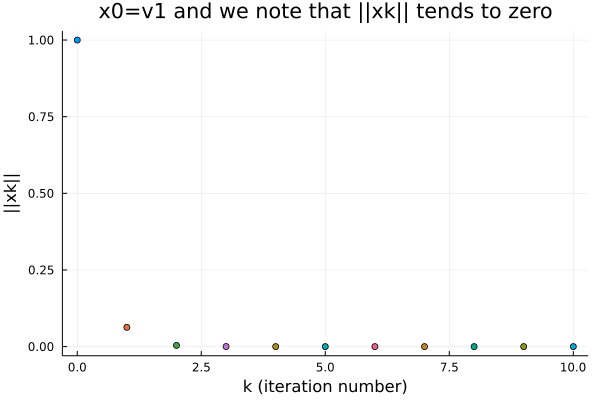
\includegraphics[width=0.6\columnwidth]{graphics/Chap08/x0Equalsv1.png} 
\end{center}

\begin{lstlisting}[language=Julia,style=mystyle]
# When x0 equals the eigenvector v3, we can observe norm(xk) goes to infinity
x = E.vectors[:,3]
p = scatter([0], [norm(x)], legend=false, xlabel="k (iteration number)", ylabel="||xk||")
for k = 1:10
    x = A*x
    # Remark xk = A^k * x0, where x0 = E.vectors[:,3]
    p = scatter!([k], [norm(x)])
end
titre="x0 = v3 and we note that ||xk|| tends to infinity"
plot!(title = titre)
png("x0Equalsv3")
display(p)
\end{lstlisting}
\textbf{Output} 
\begin{center}
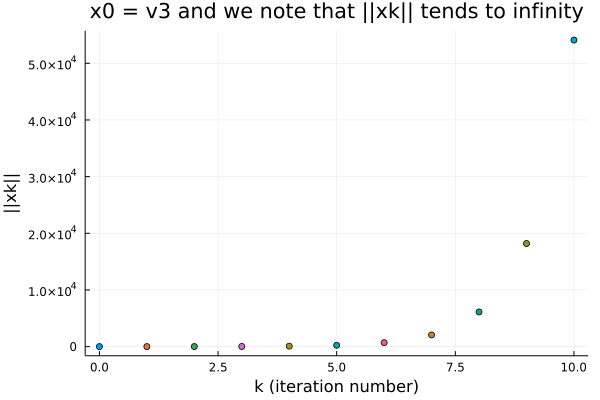
\includegraphics[width=0.6\columnwidth]{graphics/Chap08/x0Equalsv3.png} 
\end{center}

Can you ``guess'' what will happen when we take $x_0 =  2v_1+3v_3$? What happens if you add a very large quantity to a much smaller quantity? The larger quantity dominates!\\

\begin{lstlisting}[language=Julia,style=mystyle]
# What will happen when x0 = 2v1+3v3?
x = 2*E.vectors[:,1] + 3*E.vectors[:,3]
p = scatter([0], [norm(x)], legend=false, xlabel="k (iteration number)", ylabel="||xk||")
for k = 1:10
    x = A*x
    # Remark xk = A^k * x0, where x0 = 2*E.vectors[:,1] + 3*E.vectors[:,3]
    p = scatter!([k], [norm(x)])
end
titre="x0 is a linear combination of v1 and v3"
plot!(title = titre)
png("x0EqualsLinearCombov1andv3")
display(p)
\end{lstlisting}
\textbf{Output} 

\begin{center}
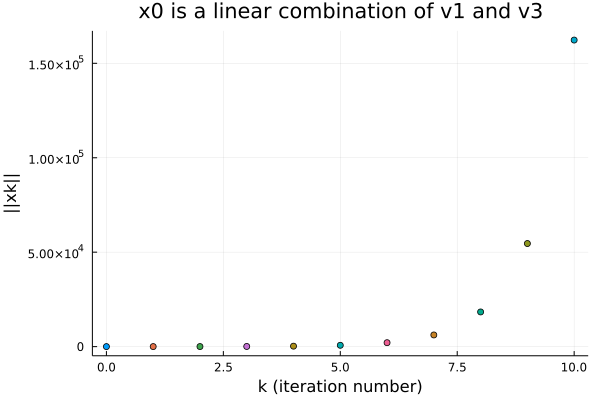
\includegraphics[width=0.6\columnwidth]{graphics/Chap08/x0EqualsLinearCombov1andv3.png} 
\end{center} 

Here is what is happening. When $x_0 = v_1$, where $v_1$ is the eigenvector corresponding to eigenvalue $\lambda_1$, we have $$x_1 = A x_0 = A v_1 = \lambda_1 v_1.$$ It follows that $$x_2 = A x_1 =  A (\lambda_1 v_1) = \lambda_1 A v_1 = (\lambda_1)^2 v_1.$$  
If $|\lambda_1| < 1$, then $(\lambda_1)^2$ is smaller and higher powers result in even smaller magnitudes.\\

In general, $x_k =  (\lambda_1)^k v_1$. Therefore, when $|\lambda_1| < 1$, $\Vert x_{k} \Vert \rightarrow 0$  as $k \rightarrow \infty$ because $|\lambda_1|^k \rightarrow 0 $ as $k \rightarrow \infty$.  Similarly, when $x_0 = v_3$, we have  $x_k =  (\lambda_3)^k v_3$. Therefore, because $|\lambda_3| > 1$, $\Vert x_{k} \Vert \rightarrow \infty$.

\begin{exercise}
Describe the set of all initial conditions $x_0$ for which $x_k$ stays bounded in our example. \\

\textbf{Hint:} The set is a two-dimensional subspace of $R^4$. \\

\end{exercise}

\textbf{Solution:} We'll call the set $S_{\rm bdd}$, where $\rm bdd$ is short for bounded. Then $$S_{\rm bdd} = \spanof{v_1, v_2} $$
because the eigenvalues associated with $v_1$ and $v_2$ have magnitude less than one. 
\Qed

\begin{exercise}
Repeat the exercise for the following matrix. \\


\textbf{Hint:} Note that the magnitude of $\lambda_1 = -3.6$ is $|-3.6| = 3.6$!

\begin{lstlisting}[language=Julia,style=mystyle]
using Random
Random.seed!(8765432123456)

# Symmetric matrices have real eigenvalues
A = randn(4, 4)
A = A+A'

# Compute eigenvalues and eigenvectors
E = eigen(A)
@show E.values
E.vectors
\end{lstlisting}
\textbf{Output} 
\begin{verbatim}
E.values = [-3.6258168896748075, -0.5790181480494843, 0.10365049366010881,
1.4790240511628157]

4×4 Matrix{Float64}:
 0.376015   0.798978  -0.133442   0.449933
 0.53203    0.223155   0.10347   -0.81021
 0.586088  -0.478348  -0.630802   0.17255
 0.481724  -0.288131   0.757348   0.333687
\end{verbatim}

\end{exercise}

\textbf{Solution:}

\begin{lstlisting}[language=Julia,style=mystyle]
# Solution here
#v1 =
#v2 = 
## PLACE YOUR SOLUTION HERE
v1 = E.vectors[:,2]
v2 = E.vectors[:,3]
[v1 v2]
\end{lstlisting}
\textbf{Output} 
\begin{verbatim}
4×2 Matrix{Float64}:
  0.0385456  -0.71411
  0.528452   -0.226828
  0.824533    0.318536
 -0.19849     0.58063
\end{verbatim}

\begin{lstlisting}[language=Julia,style=mystyle]
# To confirm this, we take a random linear combination of the vectors v1 and v2
c=randn(2,1)
x0=c[1]*v1 + c[2]*v2
# What will happen when x0 = c[1]*v1 + c[2]*v2 ????
x = x0
p = scatter([0], [norm(x)], legend=false, xlabel="k (iteration number)", ylabel="||xk||")
for k = 1:10
    x = A*x
    # Remark xk = A^k * x0, where x0 = 2*E.vectors[:,1] + 3*E.vectors[:,3]
    p = scatter!([k], [norm(x)])
end
titre="x0 is a random linear combination of v1 and v2"
plot!(title = titre)
png("x0EqualsRandomLinearCombov1andv2")
display(p)
\end{lstlisting}
\textbf{Output} 
\begin{center}
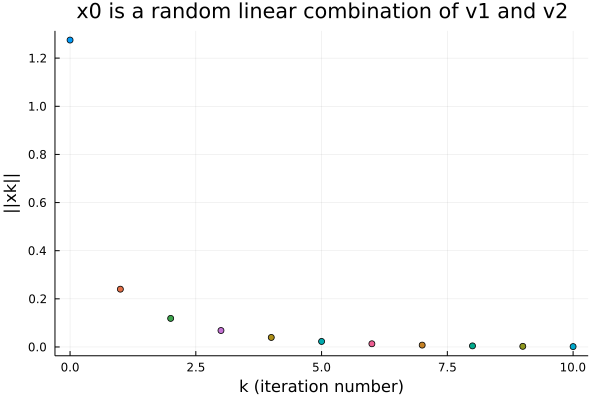
\includegraphics[width=0.6\columnwidth]{graphics/Chap08/x0EqualsRandomLinearCombov1andv2.png} 
\end{center} 




% \begin{lstlisting}[language=Julia,style=mystyle]

% \end{lstlisting}
% \textbf{Output} 
% \begin{verbatim}

% \end{verbatim}

% \begin{lstlisting}[language=Julia,style=mystyle]

% \end{lstlisting}
% \textbf{Output} 
% \begin{verbatim}

% \end{verbatim}

% \begin{lstlisting}[language=Julia,style=mystyle]

% \end{lstlisting}
% \textbf{Output} 
% \begin{verbatim}

% \end{verbatim}


% \begin{lstlisting}[language=Julia,style=mystyle]

% \end{lstlisting}
% \textbf{Output} 
% \begin{verbatim}

% \end{verbatim}

% \begin{lstlisting}[language=Julia,style=mystyle]

% \end{lstlisting}
% \textbf{Output} 
% \begin{verbatim}

% \end{verbatim}


% \begin{lstlisting}[language=Julia,style=mystyle]

% \end{lstlisting}
% \textbf{Output} 
% \begin{verbatim}

% \end{verbatim}

% \begin{lstlisting}[language=Julia,style=mystyle]

% \end{lstlisting}
% \textbf{Output} 
% \begin{verbatim}

% \end{verbatim}

% \begin{lstlisting}[language=Julia,style=mystyle]

% \end{lstlisting}
% \textbf{Output} 
% \begin{verbatim}

% \end{verbatim}


% \begin{lstlisting}[language=Julia,style=mystyle]

% \end{lstlisting}
% \textbf{Output} 
% \begin{verbatim}

% \end{verbatim}

% \begin{lstlisting}[language=Julia,style=mystyle]

% \end{lstlisting}
% \textbf{Output} 
% \begin{verbatim}

% \end{verbatim}


% \begin{lstlisting}[language=Julia,style=mystyle]

% \end{lstlisting}
% \textbf{Output} 
% \begin{verbatim}

% \end{verbatim}

% \begin{lstlisting}[language=Julia,style=mystyle]

% \end{lstlisting}
% \textbf{Output} 
% \begin{verbatim}

% \end{verbatim}

% \begin{lstlisting}[language=Julia,style=mystyle]

% \end{lstlisting}
% \textbf{Output} 
% \begin{verbatim}

% \end{verbatim}